%%%%%%%% EEML 2026 Extended Abstract — v3 (abstract-only submission) %%%%%%%%%%
\documentclass{article}
\usepackage{microtype}
\usepackage{graphicx}
\usepackage{subfigure}
\usepackage{booktabs}
\usepackage{hyperref}
\newcommand{\theHalgorithm}{\arabic{algorithm}}
\usepackage[accepted]{icml2025}
\usepackage[
  letterpaper,
  left=0.75in,
  right=0.75in,
  top=1.0in,
  bottom=1.0in,
  headheight=10pt,
  headsep=10pt
]{geometry}
\usepackage{amsmath}
\usepackage{amssymb}
\usepackage{mathtools}
\usepackage[capitalize,noabbrev]{cleveref}

\begin{document}

\twocolumn[
\icmltitle{Graph Construction from a Statistical Vocabulary}

\icmlsetsymbol{equal}{*}

\begin{icmlauthorlist}
\icmlauthor{Will Edibam}{usyd,dns}
\icmlauthor{Ben Fulcher}{usyd,dns}
\end{icmlauthorlist}

\icmlaffiliation{usyd}{The University of Sydney, Australia}
\icmlaffiliation{dns}{Dynamics and Neural Systems Group}

\vskip 0.3in
]

\begin{abstract}
Graph neural networks for multivariate time series require a relational graph that is rarely given.
Existing methods either commit to a single pairwise statistic --- discarding all other notions of dependence --- or learn edges from latent embeddings, producing opaque graphs with no statistical semantics.
We introduce a third option: parameterise graph construction over a \emph{vocabulary} of $K {\approx} 125$ named pairwise statistics spanning causal, spectral, linear, and information-theoretic families, computed via \texttt{pyspi} \citep{cliff2023}.
A learned weight vector $\mathbf{w} \in \mathbb{R}^K$, jointly optimised with a message-passing network, selects which notion of coupling is task-relevant.
We prove that any symmetric construction operator is blind to Markov-equivalent topologies; directed statistics in the vocabulary break this equivalence.
Empirically, the vocabulary achieves $100\%$ macro F1 where symmetric baselines plateau at $59\%$ and latent baselines remain at chance.
The learned $\mathbf{w}$ recovers spectral Granger causality as the dominant coupling mode --- an interpretable, testable hypothesis about the relational structure latent methods remain opaque to.
\end{abstract}

%-----------------------------------------------------------------------
\section{Introduction}
\label{sec:intro}
%-----------------------------------------------------------------------

Message-passing neural networks (MPNNs) propogate information along relational structure \citep{gilmer2017,battaglia2018}. For multivariate time series (MTS), this structure is unobserved and must be constructed from the data, and the construction choice is the critical design variable in favour of the architecture. \citet{qi2025} showed that message-passing \emph{consistently degrades} when graph construction is naive, and \citet{liu2025} found ``substantial variation'' across 239 pairwise statistics applied to the same neuroimaging data. Yet in every existing GNN pipeline, this choice is made once by the practitioner, before learning begins.

Current practice follows two regimes. The first fixes the graph from a single feature Pearson correlation for functional connectivity \citep{bullmore2009}, transfer entropy for causal graphs \citep{duan2023}. Each commits to one mathematical notion of dependence. If the task-relevant coupling is directed, nonlinear, or frequency-specific, the construction operator --- not the data --- is the bottleneck.

\textbf{The latent-embedding regime.} NRI \citep{kipf2018}, Graph WaveNet \citep{wu2019}, MTGNN \citep{wu2020}. A learned edge weight of 0.7 carries no information about \emph{what form} of dependence it represents. In scientific applications where the graph itself is the object of interest, this is a fundamental limitation.

\textbf{A provable limitation of symmetric operators.}
Consider three 3-node VAR(1) motifs: chain ($A {\to} B {\to} C$), fork ($A {\leftarrow} B {\to} C$), collider ($A {\to} B {\leftarrow} C$). Chain and fork are Markov-equivalent \citep{verma1990}: they share the same skeleton and have no v-structures, so \emph{any} symmetric statistic assigns them identical edge weights regardless of sample size. No downstream MPNN can exceed $2/3$ accuracy. Directed statistics --- where $f(X_i, X_j) \neq f(X_j, X_i)$ --- break this equivalence.

\textbf{Our approach.} We supply a \emph{vocabulary} of $K$ named pairwise statistics computed via \texttt{pyspi} \citep{cliff2023}, drawn from six complementary families: causal (transfer entropy, Granger causality, spectral GC --- \emph{asymmetric}), spectral (coherence, PLV), linear (covariance), information-theoretic (MI), distance (DTW), and rank (Spearman). A learned weight vector $\mathbf{w}$ selects which statistics are task-relevant. This follows \citet{velickovic2022}: supplying structured prior knowledge about pairwise dependence improves sample efficiency over learning relational structure from scratch.

%-----------------------------------------------------------------------
\section{Method}
\label{sec:method}
%-----------------------------------------------------------------------

Given $X \in \mathbb{R}^{M \times T}$, we compute $K$ statistics per ordered channel pair via \texttt{pyspi} \citep{cliff2023}, yielding a descriptor tensor $\mathbf{E} \in \mathbb{R}^{M \times M \times K}$. Graph construction is a linear probe of this space:
%
\begin{equation}
\label{eq:adj}
A_{ij} = \mathrm{softplus}\!\left(b + \mathbf{w}^\top \mathbf{E}_{ij}\right), \quad \text{top-}d \text{ per node}
\end{equation}
%
with $K {+} 1$ learnable parameters. The linearity is deliberate \citep[cf.][]{alain2017}: if the vocabulary is well-structured, a linear function suffices. Group lasso regularisation \citep{yuan2006} over the six SPI families encourages interpretable, family-level selection:
%
\begin{equation}
\label{eq:loss}
\mathcal{L} = \mathcal{L}_{\mathrm{task}} + \lambda_1 \|\mathbf{w}\|_1 + \lambda_g \sum_{g \in \mathcal{G}} \|\mathbf{w}_g\|_2
\end{equation}

Retained edges carry the full descriptor $\mathbf{E}_{ij}$ as attributes. An edge network $\phi(\mathbf{E}_{ij}) {=} \mathrm{MLP}(\mathbf{E}_{ij})$ conditions messages on the statistical content of each edge:
%
\begin{footnotesize}
\begin{equation}
\mathbf{m}_{ij} {=} \mathrm{MLP}\!\left(\mathbf{h}_j \| \mathbf{h}_i \| \phi(\mathbf{E}_{ij})\right)\!, \;\; \mathbf{h}_i' {=} \mathbf{h}_i {+} \mathrm{LN}\!\left(\textstyle\sum_j A_{ij}\,\mathbf{m}_{ij}\right)
\end{equation}
\end{footnotesize}
%
The vocabulary thus plays a dual role: it determines \emph{which edges exist} (via $\mathbf{w}$) and \emph{what information flows along them} (via $\phi$). Global pooling produces graph-level predictions. Training: Adam, LR warmup (60 epochs), cosine decay, restart selection (best of 2 initialisations per seed).

%-----------------------------------------------------------------------
\section{Experiments}
\label{sec:experiments}
%-----------------------------------------------------------------------

\textbf{Setup.} $M{=}10$ node VAR(1) processes ($T{=}500$) with one of three directed motifs (chain, fork, collider) embedded among 7 nuisance AR(1) channels. Coupling $\alpha \sim U(0.3, 0.7)$; 1500 instances/class; $K{=}125$ after filtering; 30 random seeds. This is a controlled test of the theory: chain and fork produce \emph{identical} symmetric pairwise statistics.

% === FIGURE 1 ===
\begin{figure*}[t]
\vskip 0.1in
\begin{center}
\subfigure[Sample efficiency]{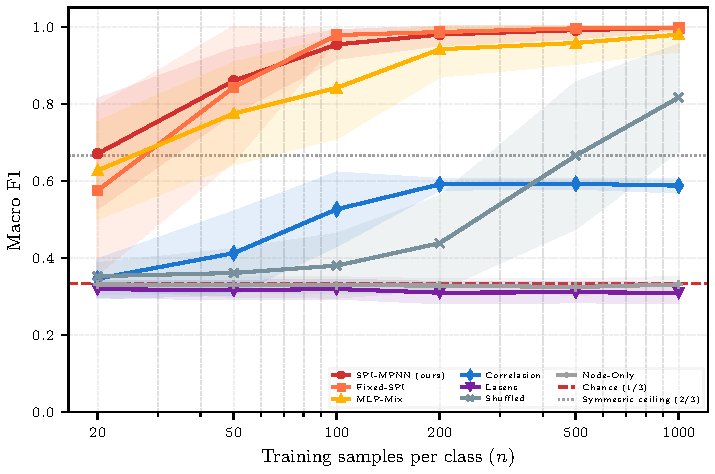
\includegraphics[width=0.62\textwidth]{figures/fig2a_sample_efficiency.pdf}\label{fig:efficiency}}
\hfill
\subfigure[Statistical signature]{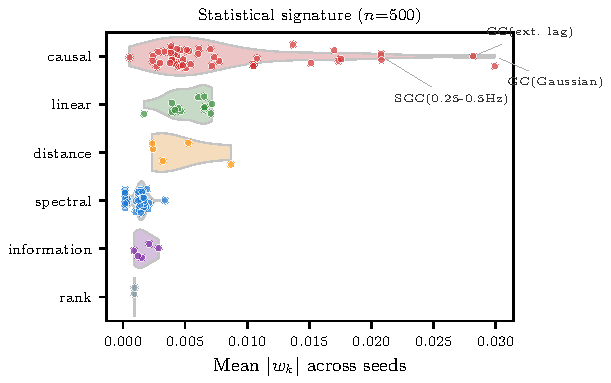
\includegraphics[width=0.35\textwidth]{figures/fig1c_family_violin.pdf}\label{fig:signature}}
\caption{(a) Vocabulary-based models reach near-perfect F1 from $n{=}100$ while Correlation plateaus below the $2/3$ ceiling and Latent remains at chance. Red dashed: $1/3$ chance; grey dotted: $2/3$ symmetric ceiling (Markov equivalence). (b) Family $L_2$ norms of learned $\mathbf{w}$ at $n{=}500$: the causal family dominates, recovering spectral Granger causality as the task-relevant coupling mode.}
\label{fig:main}
\end{center}
\vskip -0.2in
\end{figure*}

\begin{table}[ht]
\caption{Macro F1 (\%, 30 seeds, $\pm$1 s.d.).}
\label{tab:main}
\vskip 0.05in
\begin{center}
\begin{small}
\begin{tabular}{lcccccc}
\toprule
$n$/cls & SPI & Fixed & E-Abl. & Corr. & Latent & Node \\
\midrule
20   & \textbf{67}{\scriptsize$\pm$14} & 58{\scriptsize$\pm$22} & 40{\scriptsize$\pm$15}  & 35{\scriptsize$\pm$5}  & 32{\scriptsize$\pm$2} & 33{\scriptsize$\pm$2}  \\
50   & \textbf{86}{\scriptsize$\pm$8}  & 84{\scriptsize$\pm$19} & 42{\scriptsize$\pm$16}  & 41{\scriptsize$\pm$11} & 32{\scriptsize$\pm$2} & 33{\scriptsize$\pm$2}  \\
100  & 95{\scriptsize$\pm$4}  & \textbf{98}{\scriptsize$\pm$1}  & 58{\scriptsize$\pm$26}  & 53{\scriptsize$\pm$9}  & 32{\scriptsize$\pm$2} & 33{\scriptsize$\pm$2}  \\
500  & 99{\scriptsize$\pm$2}  & \textbf{100}{\scriptsize$\pm$.3}& 93{\scriptsize$\pm$11}  & 59{\scriptsize$\pm$1}  & 31{\scriptsize$\pm$2} & 32{\scriptsize$\pm$2}  \\
1000 & \textbf{100}{\scriptsize$\pm$.4}& 100{\scriptsize$\pm$.3}& 96{\scriptsize$\pm$7}   & 59{\scriptsize$\pm$2}  & 31{\scriptsize$\pm$2} & 33{\scriptsize$\pm$2}  \\
\bottomrule
\end{tabular}
\end{small}
\end{center}
\vskip -0.15in
\end{table}

\textbf{The vocabulary is the contribution, not the architecture.} All models consuming the SPI vocabulary (SPI-MPNN, Fixed-SPI) dramatically outperform all others --- the gap is not marginal but the difference between near-perfect classification and chance. Fixed-SPI, which uses the vocabulary as dense edge features on a fully connected graph with no learned topology, matches SPI-MPNN. This confirms that supplying the right \emph{representation of pairwise dependence} matters more than the mechanism used to construct edges from it. The oracle-best single statistic (spectral GC) achieves 96\% peak accuracy but with catastrophic seed failures (std up to 24\%); the full vocabulary eliminates these entirely (std ${\leq}2\%$ at $n {\geq} 50$), providing robustness through the diversity of 125 complementary estimators.

\textbf{Symmetric baselines confirm the theory.} Correlation never exceeds 59\%, well below the $2/3$ Markov-equivalence ceiling. The latent model \citep[cf.][]{wu2019} remains at chance (31--32\%) across \emph{all} sample sizes and seeds --- node-level embeddings with no statistical prior cannot access the chain--fork distinction. These are not hyperparameter failures: they are expressiveness limitations of symmetric graph construction, exactly as predicted.

\textbf{The learned $\mathbf{w}$ is an interpretable statistical signature.} Under group lasso, the causal family (48 SPIs) carries ${\sim}3.5{\times}$ the $L_2$ norm of the next family (Figure~\ref{fig:main}b). The five highest-weighted SPIs are all spectral Granger causality and time-domain Granger causality variants. For a VAR(1) process, causal structure manifests as asymmetric spectral transfer functions \citep{geweke1982} --- the model recovers this from data. An edge-ablation study (same learned topology, zeroed edge features) drops F1 to 93$\pm$11\%, confirming the MPNN uses the statistical content of edges, not merely the topology.

This is the form of output that latent graph learners cannot produce: \emph{``this task's relational structure is best captured by spectral Granger causality.''} On real-world MTS, the same mechanism would identify which notion of coupling --- coherence, transfer entropy, or combinations thereof --- is relevant to the domain, yielding interpretable graph structure directly from learned parameters.

\bibliography{references}
\bibliographystyle{icml2025}

%-----------------------------------------------------------------------
\newpage
\appendix
\onecolumn
%-----------------------------------------------------------------------

\section{Full Ablation Results}
\label{app:ablation}

Table~\ref{tab:full} provides macro F1 for all model variants. Each isolates a specific component of the method.

\begin{table}[h]
\caption{Full results (macro F1 \%, 30 seeds). SPI = SPI-MPNN, Fixed = Fixed-SPI, Mix = MLP-Mix, SGC = SGC-Only (oracle-best single SPI), E-Abl = Edge-Ablation, Corr = Correlation, Lat = Latent, Shuf = Shuffled, Node = Node-Only.}
\label{tab:full}
\vskip 0.1in
\begin{center}
\begin{small}
\begin{tabular}{lccccccccc}
\toprule
$n$/cls & SPI & Fixed & Mix & SGC & E-Abl. & Corr. & Lat. & Shuf. & Node \\
\midrule
20   & 67{\scriptsize$\pm$14} & 58{\scriptsize$\pm$22} & 63{\scriptsize$\pm$10} & 36{\scriptsize$\pm$9}  & 40{\scriptsize$\pm$15} & 35{\scriptsize$\pm$5}  & 32{\scriptsize$\pm$2} & 35{\scriptsize$\pm$3} & 33{\scriptsize$\pm$2} \\
50   & 86{\scriptsize$\pm$8}  & 84{\scriptsize$\pm$19} & 78{\scriptsize$\pm$7}  & 80{\scriptsize$\pm$18} & 42{\scriptsize$\pm$16} & 41{\scriptsize$\pm$11} & 32{\scriptsize$\pm$2} & 36{\scriptsize$\pm$6} & 33{\scriptsize$\pm$2} \\
100  & 95{\scriptsize$\pm$4}  & 98{\scriptsize$\pm$1}  & 84{\scriptsize$\pm$7}  & 87{\scriptsize$\pm$22} & 58{\scriptsize$\pm$26} & 53{\scriptsize$\pm$9}  & 32{\scriptsize$\pm$2} & 38{\scriptsize$\pm$8} & 33{\scriptsize$\pm$2} \\
200  & 98{\scriptsize$\pm$3}  & 99{\scriptsize$\pm$1}  & 94{\scriptsize$\pm$5}  & 98{\scriptsize$\pm$7}  & 75{\scriptsize$\pm$24} & 59{\scriptsize$\pm$1}  & 31{\scriptsize$\pm$3} & 44{\scriptsize$\pm$12}& 33{\scriptsize$\pm$2} \\
500  & 99{\scriptsize$\pm$2}  & 100{\scriptsize$\pm$.3}& 96{\scriptsize$\pm$5}  & ---  & 93{\scriptsize$\pm$11}& 59{\scriptsize$\pm$1}  & 31{\scriptsize$\pm$2} & 67{\scriptsize$\pm$19}& 32{\scriptsize$\pm$2} \\
1000 & 100{\scriptsize$\pm$.4}& 100{\scriptsize$\pm$.3}& 98{\scriptsize$\pm$1}  & ---  & 96{\scriptsize$\pm$7} & 59{\scriptsize$\pm$2}  & 31{\scriptsize$\pm$2} & 82{\scriptsize$\pm$14}& 33{\scriptsize$\pm$2} \\
\bottomrule
\end{tabular}
\end{small}
\end{center}
\vskip 0.1in
\textit{Note: SGC-Only entries at $n{=}500$ and $n{=}1000$ are pending.}
\end{table}

\textbf{Vocabulary ablation ladder.} The progression from single statistic to full vocabulary isolates the source of the method's advantage:

\begin{itemize}
\item \textbf{Node-Only} (33\%, chance): No pairwise features. Per-channel summary statistics (mean, std, autocorrelation, FFT peak) carry no motif information. Pairwise structure is necessary.

\item \textbf{Latent} (31--32\%, chance): Per-sample adjacency from learned node embeddings $A_{ij} = \mathrm{softplus}(\mathbf{h}_i \cdot \mathbf{h}_j / \sqrt{d})$. Symmetric by construction. Cannot access the chain--fork distinction even with unlimited data. This is an expressiveness failure, not a training failure.

\item \textbf{Correlation} (35--59\%): Fixed graph from Pearson $|r_{ij}|$. Symmetric, so provably limited to $\leq 2/3$. The gap between the theoretical ceiling and observed 59\% arises because top-$d$ sparsification selects high-correlation nuisance pairs over lower-correlation motif edges.

\item \textbf{Shuffled} (35--82\%): SPI values randomly permuted across pairs. Near chance at small $n$; rises to 82\% at $n{=}1000$ via distributional fingerprinting (SPI histograms differ across motif classes). Confirms that \emph{pair-correspondence} --- not merely the marginal distribution of SPI values --- is necessary for sample-efficient learning.

\item \textbf{Edge-Ablation} (40--96\%): Same SPI-derived adjacency as SPI-MPNN, but edge features zeroed during message passing. The 10-point gap and $3{\times}$ higher variance at $n{=}500$ (93$\pm$11\% vs 99$\pm$2\%) confirm that edge \emph{content} is load-bearing: the MPNN uses $\phi(\mathbf{E}_{ij})$ to condition messages, not merely the topology.

\item \textbf{SGC-Only} (oracle-best single SPI): Reaches 98$\pm$7\% at $n{=}200$ but with catastrophic seed failures at intermediate sizes (std 22\% at $n{=}100$, vs SPI-MPNN's 4\%). At $n{=}20$ it falls to 36\%, below Correlation. A single-statistic adjacency is fragile: the 1-dimensional edge feature provides insufficient gradient signal for reliable convergence. The full vocabulary eliminates these failures through estimator diversity.

\item \textbf{MLP-Mix} (63--98\%): Nonlinear adjacency $A_{ij} = \sigma(\mathrm{MLP}(\mathbf{E}_{ij}))$. Functional but no advantage over the linear $\mathbf{w}$, validating the linear probe design: the vocabulary is sufficiently well-structured that linearity suffices.

\item \textbf{Fixed-SPI} (58--100\%): Fully connected graph with $\mathbf{E}_{ij}$ as dense edge features. Matches or exceeds SPI-MPNN at $n \geq 100$. This is a key finding: the vocabulary provides sufficient information as edge features for an MPNN to learn effective relational reasoning, even without learned topology. The advantage of SPI-MPNN is interpretability via $\mathbf{w}$, not raw accuracy.
\end{itemize}

\section{Top Learned Weights}
\label{app:weights}

Under group lasso ($\lambda_g{=}0.02$, $\lambda_1{=}0.001$), the five highest mean $|w_k|$ across 30 seeds at $n{=}500$:

\begin{table}[h]
\begin{center}
\begin{small}
\begin{tabular}{llc}
\toprule
SPI & Family & $\overline{|w_k|}$ \\
\midrule
SGC parametric mean (0.25--0.5\,Hz, order 1) & Causal & 0.0226 \\
GC Gaussian ($k{=}1$, $l{=}1$) & Causal & 0.0225 \\
GC Gaussian (extended lag) & Causal & 0.0206 \\
SGC parametric max (0.25--0.5\,Hz, order 1) & Causal & 0.0202 \\
SGC parametric mean (0.25--0.5\,Hz, free order) & Causal & 0.0141 \\
\bottomrule
\end{tabular}
\end{small}
\end{center}
\end{table}

All five are directed temporal measures. For a VAR(1) generating process, the causal structure manifests as asymmetric spectral transfer functions in exactly the 0.25--0.5\,Hz band --- the model recovers this from data. The linear and distance families retain moderate weight (Figure~\ref{fig:main}b), consistent with their role as general coupling detectors, while information and rank families are driven near zero by the group lasso.

\end{document}
